% Chapter 9

\chapter{YoMap Matlab User Guide} % Main chapter title

\label{Chapter9} % For referencing the chapter elsewhere, use \ref{Chapter1} 

\lhead{Chapter 9. \emph{YoMap Matlab User Gude}} % This is for the header on each page - perhaps a shortened title

%----------------------------------------------------------------------------------------

\section{Introduction}
	YoMap Matlab is an open source map for city Le Creusot . It was developed by a group of ViBOT/MsCV students with using MATLAB R2013a. YoMap contains the basic data and functions that can help you to orient in the city. In this guide you will find instructions on using the YoMap.
	
For any questions free welcome to contact:
Ozan: emreozanalkan@gmail.com
Klemen: klemen.istenic@gmail.com 
Oksana:	oksana.hagen@gmail.com
Natalia: natalia.shepel@gmail.com
\begin{center}
Enjoy of using!
\end{center}

	
\section{Getting Started}
	Program window is represented on figure \ref{fig:1}. Elements of map:
	\begin{enumerate}
		\item Layers Panel
		\item Instruction Panel
		\item Search Panel
		\item Hide Button
		\item Info Button
		\item Map Manipulation Panel
		\item Map
	\end{enumerate}
	
	For zoom in, zoom out or pan map click on the corresponding icons on the map manipulation panel. 
	
	All information about way and point interest is represented on the Introduction panel. 
	
	To hide/show map, roads, categories and way use layers panel. All changes will be shown on the map. 
	
	Search parameters can be changed on the search panel. Use button "hide all" to hide/show search panel.
	
	Press "info" to see information about map.
  \begin{figure}[h]
  \centering
  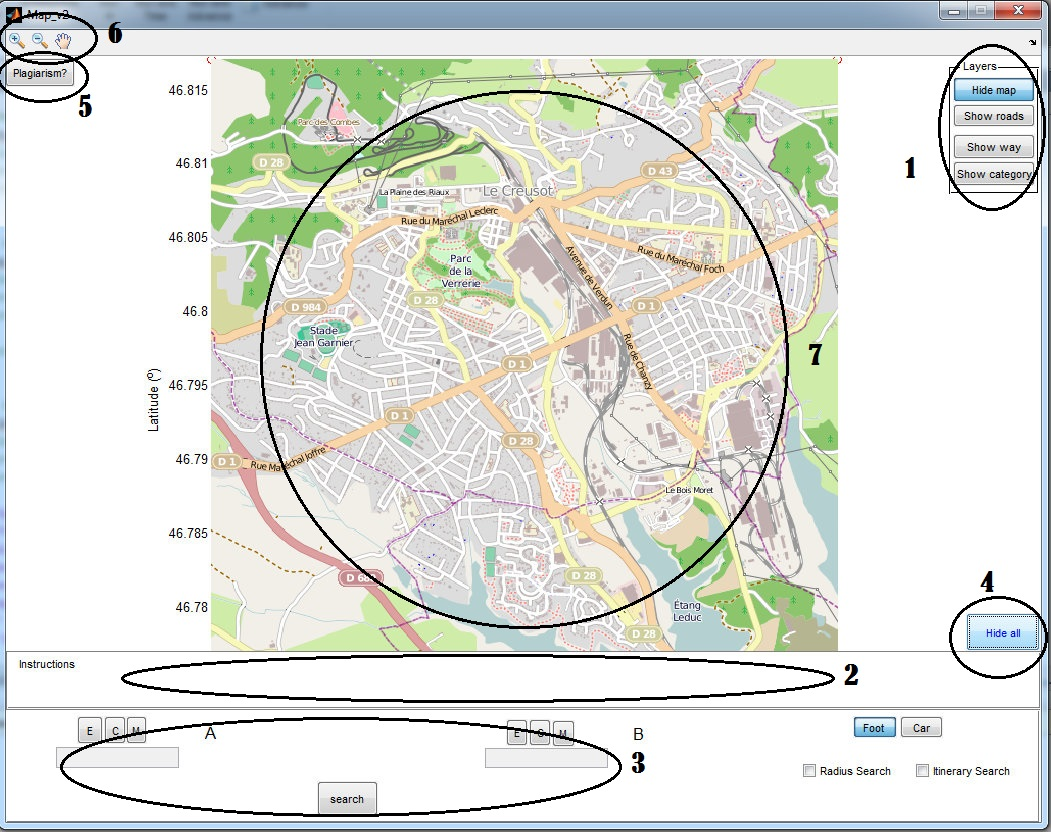
\includegraphics[ width=0.8\textwidth]{../pictures/1.jpg}
  \caption{Yomap MATLAB GUI}
			\label{fig:1}
  \end{figure}
  
\section{Data Entry}
		To start search choose one of the tabs on the search panel (figure \ref{fig:2}):
		
		\begin{enumerate}
			\item Enter Tab - allows choosing object by category and name
			\item Category Tab - allows choosing object by category and name
			\item Show On Map Tab - allows either pick any point on the map or either enter coordinates manually
		\end{enumerate}
		
		In case of choosing layer "Show Category" any existing object can be chosen either manually or either with a mouse click (figure \ref{fig:3}).
		To pick point with a mouse click button "Pick" and choose any exciting object. The dot, representing object will appears (figure \ref{fig:4}). Please be very precise.
	  \begin{figure}[h]
	  \centering
	  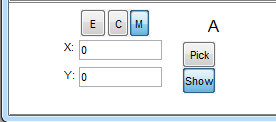
\includegraphics[ width=0.8\textwidth]{../pictures/2.jpg}
	  \caption{Search panel}
				\label{fig:2}
	  \end{figure}
	  	  \begin{figure}[h]
	  	  \centering
	  	  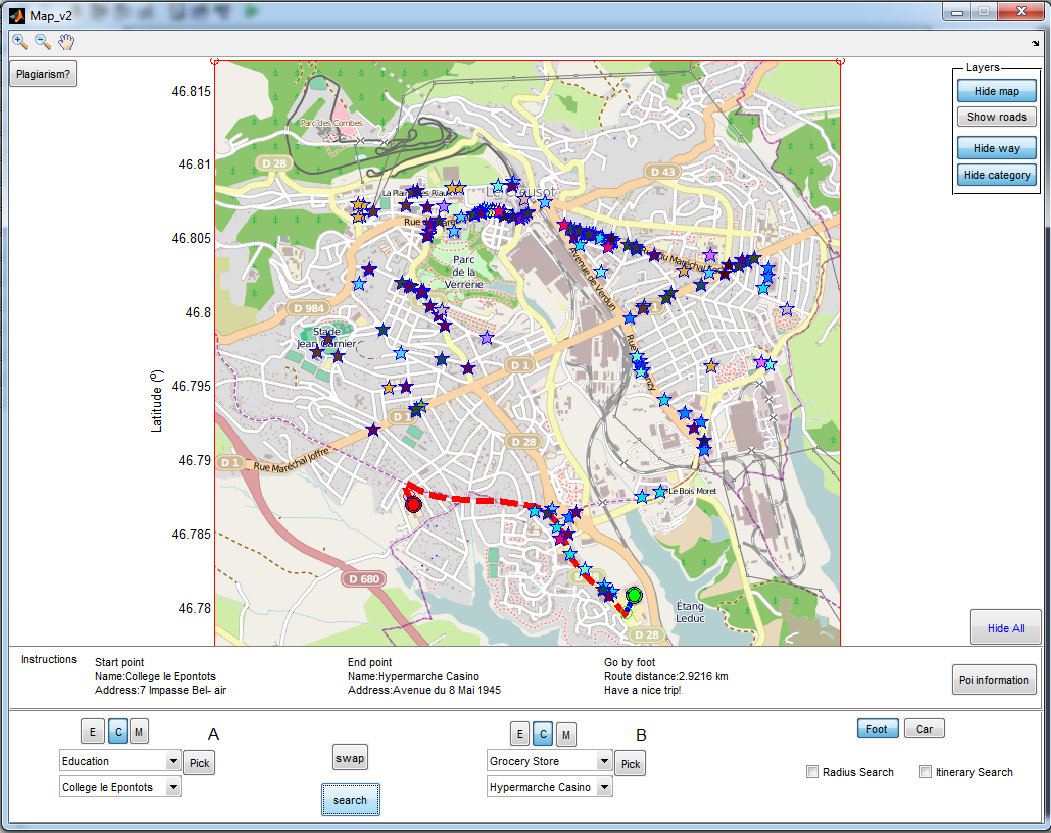
\includegraphics[ width=0.8\textwidth]{../pictures/3.jpg}
	  	  \caption{Enter data}
	  				\label{fig:3}
	  	  \end{figure}
	  	  	  \begin{figure}[h]
	  	  	  \centering
	  	  	  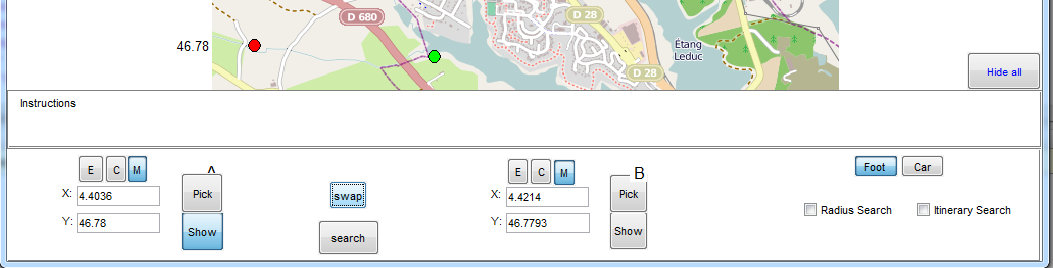
\includegraphics[ width=0.8\textwidth]{../pictures/4.jpg}
	  	  	  \caption{The dot representation}
	  	  				\label{fig:4}
	  	  	  \end{figure}
\section{Layers Usage}
	To show/hide any additional map information – press corresponding layer button on the layer panel (figure \ref{fig:5}). Be careful. In case if there is no way "Show Way" will not work.
 	  \begin{figure}[h]
 	  \centering
 	  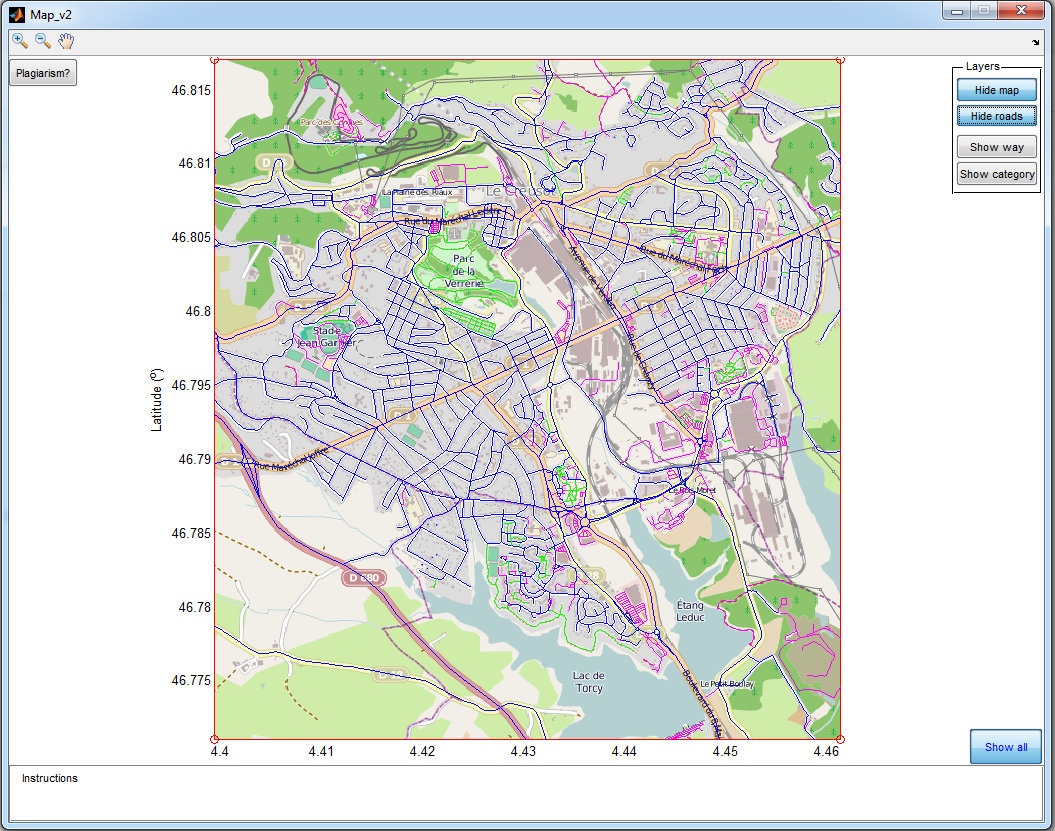
\includegraphics[ width=0.8\textwidth]{../pictures/5.jpg}
 	  \caption{Layer panel}
  	  				\label{fig:5}
 	  \end{figure}
\section{Point of Interest Information}
	To see any information about existing objects press first "Show Category" button. After this "point information" button will appears on the instruction panel. To see information about point click button and choose any exciting object. Information about point will appears on the instruction panel (figure \ref{fig:6}). Please be very precise.
	\begin{figure}[h]
	\centering
	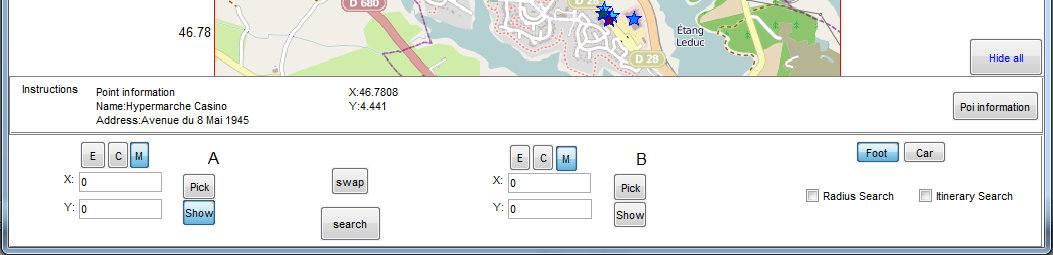
\includegraphics[ width=0.8\textwidth]{../pictures/6.jpg}
	\caption{Instruction panel}
		  				\label{fig:6}
	\end{figure}
\section{Shortest Path Search}
	To find shortest path between 2 points choose any tab for each point in search panel. Enter information and press "Search" button.  All information about way will appears on the instruction panel (figure \ref{fig:7}) and path will be shown on the map.
	In case if same tabs for both point will be pushed, button "Swap" will appear (figure \ref{fig:8}). Use it to swap points on the map.
		\begin{figure}[h]
		\centering
		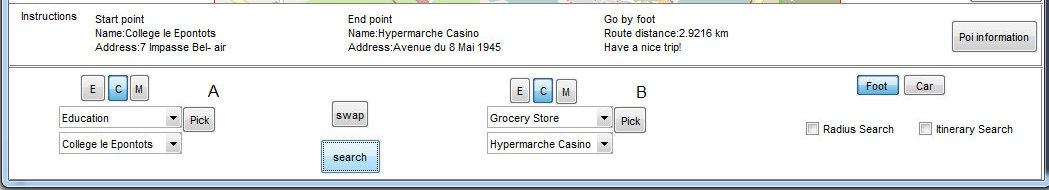
\includegraphics[ width=0.8\textwidth]{../pictures/7.jpg}
		\caption{Instruction panel}
			  				\label{fig:7}
		\end{figure}
	\begin{figure}[h]
	\centering
	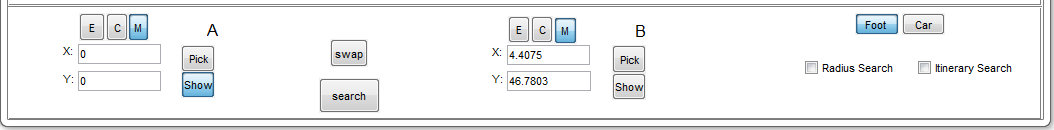
\includegraphics[ width=0.8\textwidth]{../pictures/8.jpg}
	\caption{Swap button}
		  				\label{fig:8}
	\end{figure}
\section{Shortest Path Search With a Middle Point}
	To find path with a middle point click on the "Itinerary Search" on the search panel. Middle point and textbox for enter distance will appear (figure \ref{fig:9}). Enter information for start and end point and choose category from the menu of middle point. Write required search distance in kilometres. Be carefully:  0 distance corresponds to unlimited distance search. Press button "Search". The closest object from category in middle point will be chosen. All information about way will appears on the instruction panel and path will be shown on the map.
		\begin{figure}[h]
		\centering
		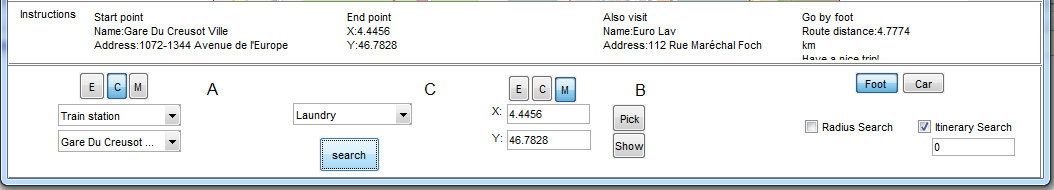
\includegraphics[ width=0.8\textwidth]{../pictures/9.jpg}
		\caption{Shortest Path Search With a Middle Point}
			  				\label{fig:9}
		\end{figure}
\section{Radius Search}
	To find closest object to initial point from category press the "Radius search". Textbox for enter distance will appear (figure 9). Enter information for start point and choose. Write required search distance in kilometers. Be carefully:  0 distance corresponds to unlimited distance search. Press button "Search". The closest object from category will be chosen. All information about way will appears on the instruction panel and path will be shown on the map.
		\begin{figure}[h]
		\centering
		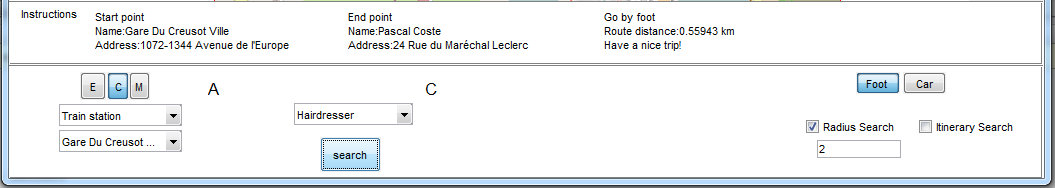
\includegraphics[ width=0.8\textwidth]{../pictures/10.jpg}
		\caption{Radio search}
			  				\label{fig:10}
		\end{figure}	